\section{Objectifs du cours}
La Mécanique des Milieux Continus (MMC) est l'étude de milieux solides ou fluides qui \textbf{se déforment}. Par exemple, la déformation d'une balle lorsqu'on la compresse, le choc entre deux tuyaux, ... La MMC est donc une bonne introduction pour la Mécanique des Fluides et la Mécanique des Solides Déformables car elle va nous donner un tas d'outils mathématiques pour analyser et résoudre des équations de déformations.


\textcolor{red}{à développer}
%TODO

\section{Volumes élémentaires représentatifs}
Lorsqu'on souhaite caractériser une grandeur physique dans un solide complexe (e.g., la masse volumique), on peut utiliser des VER (volumes élémentaires représentatifs). 
\begin{figure}[H]
    \centering
    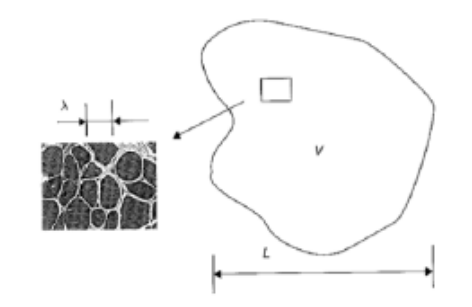
\includegraphics[scale = 0.75]{Images/Images_Introduciton/VER_Schema.png}
    \caption{Illustration d'un VER \protect\footnotemark}
    \label{fig:my_label}
\end{figure}
\footnotetext{Image tirée des slides "introduction", version 2017}
Le principe est le suivant : On prend un "petit morceau" du volume afin de représenter les propriétés moyennes du matériau. Ce morceau doit être suffisamment grand pour qu'il  représente correctement la structure du matériau et assez petit que pour qu'il puisse être mathématiquement considéré comme un point mais pas comme une molécule ou un atome.

\begin{figure}[H]
    \centering
    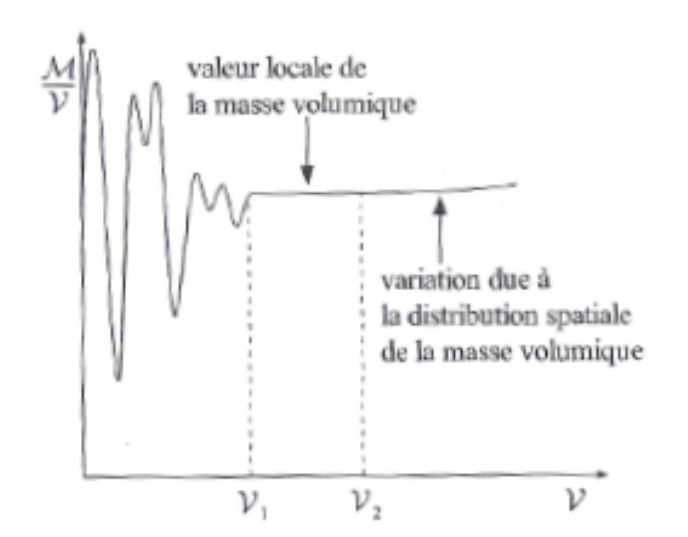
\includegraphics[scale = 0.5]{Images/Images_Introduciton/VER_Graphe.png}
    \caption{Fluctuation de la masse volumique en fonction du volume de l'élément \protect \footnotemark}
    \label{fig:fluctuationsVER}
\end{figure}
\footnotetext{Image tirée des slides "introduction", version 2017}

Pour trouver la grandeur en un point du solide, on fera la moyenne de cette grandeur sur un élément de volume l'entourant. De plus, dans cette moyenne, on se servira du modèles à une échelle inférieur. (e.g., échelle cristalline, moléculaire)\\
\\
Par exemple : Si nous souhaitons calculer la masse volumique d'un solide en un point P.
\begin{enumerate}
    \item On choisi un élément de volume de taille adéquate
    \item On calcul la moyenne de la masse volumique sur cet élément de volume en suivant le modèle cristallin
    \item La masse volumique du solide au point P vaudra la moyenne calculée à l'étape 2.
\end{enumerate}
Comme on le voit sur la figure \ref{fig:fluctuationsVER}, Si le volume de l'élément est inférieur à $V_1$, la masse volumique de l'élément ne sera plus représentative de la masse volumique du solide. Pour une faible variation de volume, la masse volumique variera de manière non-négligeable. En revanche, si le volume est supérieur à $V_1$, la masse volumique sera presque constante. Il nous faut donc choisir une taille de VER telle que $\lambda << VER << V$, où $\lambda$  est de taille infiniment petite et V est le volume total de notre Milieu Continu.\\

\section{Les hypothèses de la MMC}

\begin{itemize}
    \item Les lois ne sont pas modifiées si on change d'observateur
    \item Les lois ne sont pas modifiées si on change le systèmes de coordonnées.
    \item Les lois sont les mêmes partout dans l'espace et dans le temps.
    \item L'espace est euclidien ($\mathbb{R}^3$ muni d'un produit scalaire)
\end{itemize}


